\documentclass[12pt,a4paper]{article} % 注意:article 不支持 15pt,最大 12pt
\usepackage{amsmath}
\usepackage{amssymb}
\usepackage{notex}
\usepackage{tikz}
\usepackage{graphicx}
\usepackage{float}
%\usepackage[useregional]{datetime2}
\usepackage{float}
\usepackage{tikz-3dplot}
\usepackage{xcolor}
\usepackage[justification=centering]{caption}
\usepackage{makecell,rotating,multirow,diagbox}
\usepackage{pgfplots}
\pgfplotsset{compat=1.18}
\usepackage{ctex}
\usepackage{fontspec}
% \setCJKmainfont{Noto Sans CJK SC}
% \setCJKsansfont{Noto Sans CJK SC}
% \setCJKmonofont{Noto Sans CJK SC}

\setmainfont{TeX Gyre Termes}

\usepackage{geometry}
\geometry{left=0.5cm,right=0.5cm,top=3cm,bottom=3cm}
\usepackage{setspace}
\renewcommand{\baselinestretch}{1.245}

\usepackage{fancyhdr}
\pagestyle{fancy}
\fancyhf{}
\lhead{\large\textbf{湖南大学}}
\fancyhead[C]{\includegraphics[width=0.05\textwidth]{/home/zqj/Downloads/image-removebg-preview.png}}
\rhead{课程笔记}
\cfoot{\thepage}
\lfoot{$\mathfrak{ONLY\ USED\ BY\ VIP}$}
\rfoot{$copyright\ belongs\ to\ zqj$}
\usepackage{enumitem}

\title{历史课笔记:马克思主义传播与中共早期组织的形成}
\author{705  周全景}
\date{\today}


\begin{document}

\maketitle
\tableofcontents
\clearpage

\vspace*{5cm}
\begin{figure}[H] 
	\centering
	\includegraphics[width=0.5\textwidth]{/home/zqj/Downloads/image-removebg-preview.png} % example-image 为测试图片(无需实际文件)
	\caption\textbf{\large\color{red}{千年学府,百年名校}}
	\label{fig:example}
\end{figure}


\newpage

\section{马克思主义的诞生与传播}
	\subsection{五四运动与新文化运动}
		\begin{itemize}
			\item{1899年《万国公报》第一个宣传马克思主义,士农\gl{工}商,"工"不指工人而是手工业者。}
			\item 日本成为马克思主义向中国传播的主要途径,中国赴日留学增多,孙中山领导的革命党人和无政府主义者是早期传播的重要力量,日本译作
			\item 梁启超最早介绍马克思主义
			\item \gl{然而}:陈独秀认为“产业未兴,兼并未盛”,条件不足,时机未到
		\end{itemize}

	\subsection{马克思主义的诞生}
		\subsubsection{要解决的问题}
			资本家和工人阶级的矛盾
		
		\subsubsection{对社会主义革命的研判}
			革命会发生在生产力发达的资本主义国家
			\begin{enumerate}
				\item 这里矛盾最尖锐
				\item 商品经济充分发展
				\item 工人阶级队伍壮大,战斗力强
			\end{enumerate}
		\subsubsection{观点}
			同时革命论。不认可太平天国运动,没有提高生产力,推动工业化

\newpage

\section{马克思主义在中国的广泛传播}
	\subsubsection{国际因素}
		\begin{enumerate}
			\item 第一次世界大战打破“欧风美雨”
			\item 十月革命爆发
			\item 巴黎和会中国外交失败
		\end{enumerate}
	\subsubsection{国内因素}
		五四运动,中国工人阶级第一次登上历史舞台
	\subsubsection{两大特点}
		\begin{itemize}
			\item 传播途径更广
			\begin{enumerate}
				\item 各类译作
				\item 勤工俭学向国内发通讯
				\item 赴俄留学生:传播俄国革命经验主要力量
				\item 第三国际的干预
			\end{enumerate}
			\item 传播内容更丰富
			\begin{enumerate}
				\item 社会存在决定社会意识,\gl{而不是}“天道不变”
				\item 人民群众是历史创造者(\gl{与陈独秀改造国民有不同})
				\item {阶级和阶\color{red}级斗争的观点}(\gl{有不同})
				\item 国家是阶级的统治工具
			\end{enumerate}
		\end{itemize}

\newpage

\section{马列主义在中国的广泛传播}
	\begin{itemize}
		\item 苏俄危机$\implies$严峻外部环境
		\item 战后工人运动$\implies$列宁号召{\color{green}世界革命}
		\item $1919\text{年}03\text{月}02\text{日}\sim 06\text{日}$,第三国际,世界苏维埃社会主义共和国联盟
		\item 威联斯基,《新青年》成为“\rm{Soviet Russia}的汉译本”
	\end{itemize}

\newpage

\section{早期马克思主义者的产生}
	\subsubsection{陈独秀等最早的一批}
		主要是学生

		改良$\longrightarrow $革命,思想突变
			\begin{itemize}
				\item 俄国$\leftarrow$ 陈独秀:《谈政治》
				\item 日本$\leftarrow$ 李大钊:《我的马克思主义观》
			\end{itemize}
	\subsubsection{法国勤工俭学群体}
		蔡和森,周恩来......
	\subsubsection{革命党群体}
		希望找到新路子

		董必武......
	
	\newpage
	

	% \begin{tabular}{|c|c|r|}
	% 	\hline
	% 	q & 1 & hthty \\
	% 	\hline
	% 	qq & tyrtfdsffifjoisfosgifgfogsbfkbskbfmbskglghgls & fdfsdv \\
	% 	\hline
	% \end{tabular} \\
	% \wryh{太阳有多大} \\

	% \td{what to do}


	% % 方式1:直接插入(适合小图)
	% \begin{center}
	% 	\begin{tikzpicture}
	% 		\draw[->] (0,0) -- (3,0) node[right] {$x$};
	% 		\draw[->] (0,0) -- (0,3) node[above] {$y$};
	% 		\draw[->, thick, red] (0,0) -- (2,1.5) node[midway, below right] {$\vec{v}$};
	% 	\end{tikzpicture}
	% 	\label{first}
	% \end{center}

	% % 方式2:用 figure 环境(推荐,可加标题和浮动)
	% \begin{figure}[H]
	% 	\centering
	% 	\begin{tikzpicture}
	% 		\draw[->] (0,0) -- (3,0) node[right] {$x$};
	% 		\draw[->] (0,0) -- (0,3) node[above] {$y$};
	% 		\draw[->, thick, blue] (0,0) -- (2,1.5) node[midway, above left] {$\vec{v}$};
	% 	\end{tikzpicture}
	% 	\caption{一个二维矢量示意图}
	% 	\label{fig:vector}
	% \end{figure}
	% \begin{figure}
	% 	\begin{center}
	% 		\tdplotsetmaincoords{60}{110} % 设置视角:仰角60°,方位角110°
	% 		\begin{tikzpicture}[scale=2, tdplot_main_coords]
	% 		% 坐标轴
	% 			\draw[->, thick] (0,0,0) -- (1.5,0,0) node[anchor=north east]{$x$};
	% 			\draw[->, thick] (0,0,0) -- (0,1.5,0) node[anchor=north west]{$y$};
	% 			\draw[->, thick] (0,0,0) -- (0,0,1.5) node[anchor=south]{$z$};

	% 			% 三维矢量 v = (1, 1, 1)
	% 			\draw[->, thick, red] (0,0,0) -- (1,1,1) node[midway, above right]{$\vec{v}$};

	% 			% 可选:投影到 xy 平面
	% 			\draw[dashed, gray] (1,1,0) -- (1,1,1);
	% 			\draw[dashed, gray] (0,0,0) -- (1,1,0);
	% 		\end{tikzpicture}
	% 	\end{center}
	% 	\caption{$\mathfrak{GOOD\_3D}$}
	% \end{figure}

	% \vspace*{3cm}
	
	% $\mathit{x1_e+d}$
	\vspace*{3cm}
	\begin{tikzpicture}
	\begin{axis}[
		ybar,
		bar width=30pt,          % ← 修正拼写
		xlabel={类别},
		ylabel={数值},
		xtick={1,2,3,4},
		xticklabels={A,B,C,D},
		ymin=0,
		ymax=100,
		width=15cm,
		height=10cm
	]
	\addplot coordinates {(1,30) (2,70) (3,50) (4,90)}; % ← 添加数据
	\end{axis}
	\end{tikzpicture}

	\vspace*{3cm}
	\begin{center}
	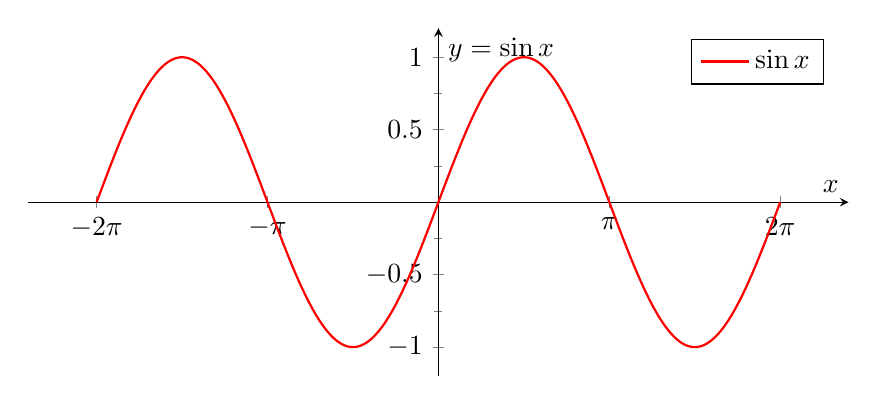
\begin{tikzpicture}
	\begin{axis}[
		xlabel={$x$},
		ylabel={$y = \sin x$},
		minor tick num=1,
		width=12cm,
		height=6cm,
		domain=-2*pi:2*pi,
		samples=200,
		axis lines=middle,
		enlargelimits=true,
		xtick={-6.283,-3.1416,0,3.1416,6.283},
		xticklabels={$-2\pi$,$-\pi$,0,$\pi$,$2\pi$},
		ytick={-1,-0.5,0,0.5,1},
		legend pos=north east
	]
	\addplot [thick, red] {sin(deg(x))};
	\legend{$\sin x$}
	\end{axis}
	\end{tikzpicture}
	\end{center}

	\begin{center}
		\begin{tikzpicture}
			\begin{axis}
				xlabel={kl}
				ylabel={what\ can\ i\ say}
				width=15
				height=10
				domain=-2*pi:2*pi
				samples=500
				xtick=-6.28,-3.14,0,3.14,6.28
				xticklabels={$2\pi,-\pi,0,\pi,2\pi$}
				ytick={-2,-1,0,1,2}
				legendpose=north east
				\addplot[thick,red] {cos(x)}
			\end{axis}
			
		\end{tikzpicture}
		
	\end{center}

\end{document}
